\documentclass[12pt,a4paper]{article}
\usepackage[UTF8]{ctex}
\usepackage{graphicx}
\usepackage{geometry}
\usepackage{ulem}
\usepackage{enumitem}
\usepackage{titlesec}
\usepackage{multicol}
\usepackage[export]{adjustbox}
\usepackage{amsmath}  % 推荐用于更好的数学排版
\usepackage[utf8]{inputenc}
\usepackage{CJKutf8}
\usepackage{fancyhdr}
\usepackage{lastpage}
\usepackage{ulem}
\usepackage{tabularx}
\usepackage{lastpage}
\usepackage{float}
\usepackage{circuitikz}
\usepackage{array}
\usepackage{subcaption}
% 页眉页脚设置
\pagestyle{fancy}
\fancyhf{} % 清除所有页眉页脚
% 设置页眉内容
%-==========1. 填写从第二页开始 每页第一行的信息==========-
\fancyhead[C]{
    \makebox[4.5em][c]{实验名称：} \uline{\makebox[14em][c]{集成运算放大器应用电路研究(I)}} 
    \makebox[2.5em][c]{姓名：} \uline{\makebox[4em][c]{}} 
    \makebox[2.5em][c]{学号：} \uline{\makebox[5em][c]{}}
}%--------------------------------------------------------
\fancyfoot[C]{第 \thepage\ 页，共 \pageref{LastPage} 页}

% 取消页眉和页脚的下划线
\renewcommand{\headrulewidth}{0pt} % 页眉横线粗细设为0
\renewcommand{\footrulewidth}{0pt} % 页脚横线粗细设为0

% 调整页眉高度
\setlength{\headheight}{50pt}

% 设置plain样式（用于第一页）
\fancypagestyle{plain}{
    \fancyhf{} % 清除所有页眉页脚
    \renewcommand{\headrulewidth}{0pt} % 隐藏页眉横线
    \fancyfoot[C]{第 \thepage\ 页，共 \pageref{LastPage} 页} % 保留页脚
}
% 设置页面边距
\geometry{left=2.54cm,right=1.5cm,top=2.54cm,bottom=2.54cm}

% 设置正文字体大小为小四
\renewcommand{\normalsize}{\fontsize{12pt}{18pt}\selectfont}
% 设置章节格式
\titleformat{\section}{\fontsize{16pt}{24pt}\selectfont\bfseries}{\thesection}{1em}{} % 一级标题：三号
\titleformat{\subsection}{\fontsize{15pt}{22.5pt}\selectfont\bfseries}{\thesubsection}{1em}{} % 二级标题：小三

\begin{document}
\thispagestyle{plain}%第一页使用 plain 样式，而不是默认的 fancy 样式，第一页不再显示页眉
% 标题部分 - 两栏布局
\begin{multicols}{2}
    % 左栏：图片和实验报告标题
    % 左栏：使用空行创建前三行
    \noindent
    ~\\ % 第一行
    ~\\ % 第二行
    ~\\ % 第三行
    \hphantom{占位}% 使用空占位符
    \raisebox{-0.5\baselineskip}% 图片向下移动半行
    {
\includegraphics[width=1.85in,height=0.58in]{figure/ZJU.jpg}}
    \hspace{.5em}% 图片和标题之间的间距
    \raisebox{0pt}[\height][0pt]% 标题底部对齐
    {\textbf{\fontsize{26pt}{30pt}\selectfont 实验报告}}
    
    \columnbreak % 换到右栏
    
    % 右栏：个人信息
    % 右栏：个人信息 - 靠右对齐 
%-==========2. 填写个人信息==========-
    \begin{flushright}
        \makebox[3em][l]{专业：} \uline{\makebox[9em][c]{}} \\
        \makebox[3em][l]{姓名：} \uline{\makebox[9em][c]{}} \\
        \makebox[3em][l]{学号：} \uline{\makebox[9em][c]{}} \\
        \makebox[3em][l]{日期：} \uline{\makebox[9em][c]{2025年12月16日}} \\
        \makebox[3em][l]{地点：} \uline{\makebox[9em][c]{紫金港东四216}} \\
    \end{flushright}   
\end{multicols}
% 课程名称等信息（单栏）
%-==========3. 填写课程信息==========-
\noindent\small
课程名称： \uline{电子电路设计实验I} \hfill 指导老师： \uline{施红军、叶险峰、邓靖靖} \hfill 成绩： \uline{\hspace{3cm}} \\
实验名称： \uline{集成运算放大器应用电路研究(I)} \hfill 实验类型： \uline{设计类实验} \hfill 同组学生姓名： \uline{}
%-==========4. 正文开始==========-
\section*{一、实验目的}
1.研究由集成运放构成的比例、加法、减法等基本运算电路的组成与功能，加深对集成运放线性应用电路结构和性能特点的理解，掌握其设计方法。

2.研究放大电路增益带宽积与单位增益带宽的关系。

3.了解运算放大器构成的基本运算电路在实际应用时的局限性和应考虑的问题。

\section*{二、实验任务与要求}
1.设计、研究反相放大器

2.设计安装算术运算电路

3.研究增益带宽积

\section*{三、实验原理}
1. 集成运放概述

集成运算放大器（简称集成运放）是一种高电压增益、高输入电阻、低输出电阻、直接耦合的多级放大集成电路。由于集成运放具有极高的差模电压增益，要使其稳定工作于线性区，必须加深度负反馈，否则它将工作于饱和区或非线性状态。

在运放输出端与输入端之间接不同的反馈网络，可实现不同用途的电路：信号放大、信号运算、信号处理（滤波、调制）、波形产生和变换等。反馈，就是把输出回路中的电压或电流，通过一定的电路（反馈网络）送回到放大器的输入回路的过程。如果反馈到输入回路中去的电量是对输入信号起抵消作用，结果使闭环放大倍数减小的，称为负反馈。反之，称为正反馈。根据反馈信号在输入回路中的连接方式，可以分为串联反馈和并联反馈；根据反馈信号在输出回路中的采样方式，可以分为电压反馈和电流反馈。

在分析或设计集成运放构成的电路时，通常可认为运放是“理想的”，其理想化参数为：

	输入阻抗 \(R_i = \infty\); 	开环差模电压增益 \(A_{vd} = \infty\);

    输出阻抗 \(R_o = 0\);		共模抑制比 \(CMRR = \infty\);

    带宽 \(BW = \infty\);		失调、温漂等均为零。

2. 理想运放在线性区的两个重要特性

由于理想运放的参数特性，当运放工作于深度负反馈构成的线性区时，可以得出以下两个重要结论，它们极大地方便了电路的分析：
\begin{itemize}
	\item \textbf{虚短}： 由于 \(A_{vd} = \infty\)，而输出电压为有限值，因此同相输入端与反相输入端之间的电压差趋于零，即 \(u_+ - u_- \approx 0\) 或 \(u_+ \approx u_-\)。
	\item \textbf{虚断}： 由于 \(R_i = \infty\)，流入运放同相输入端和反相输入端的电流趋于零，即 \(i_+ \approx 0\)， \(i_- \approx 0\)。
\end{itemize}

3. 基本运算放大电路

基于理想运放模型和“虚短”、“虚断”概念，可以方便地分析各种运放应用电路。


(1) \textbf{反相比例放大器}
\begin{itemize}
	
\begin{figure}[H]
    \centering
    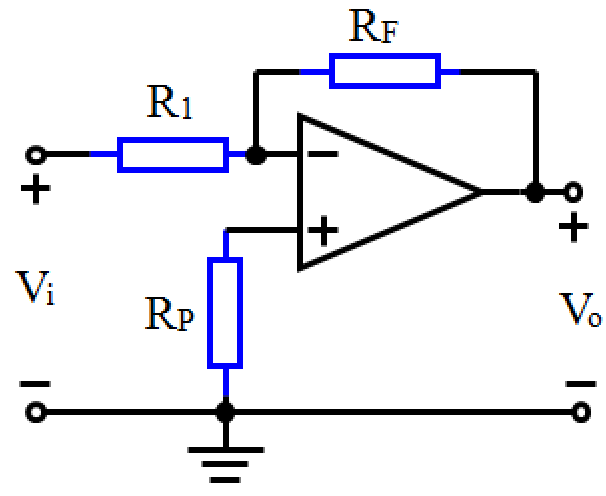
\includegraphics[width=0.4\textwidth, height=0.2\textheight]{figure/circuit_1.png}
    \caption{反相比例放大电路}
    \label{fig:inverting_amp}
\end{figure}


	\item \textbf{电压增益 \(A_v\)}： 根据“虚短”（\(v_- \approx v_+ = 0\)）和“虚断”（\(i_- \approx 0\)），有 \(i_1 = i_2\)。 解得：
	      \[
		      A_v = \frac{v_o}{v_i} = -\frac{R_f}{R_1}
	      \]
	      输出电压与输入电压成比例关系，且相位相反。
	\item \textbf{输入电阻 \(R_{i}\)}： 由于反相输入端为“虚地”（\(u_- \approx 0\)），从信号源看进去的输入电阻近似为：
	      \[
		      R_{i} \approx R_1
	      \]
	\item \textbf{输出电阻 \(R_{o}\)}： 在理想运放和深度电压负反馈条件下，输出电阻趋于零：
	      \[
		      R_{o} \approx 0
	      \]
\end{itemize}

$R_p$一般取$R_1||R_f$，以减小输入偏置电流引起的运算误差。

(2) \textbf{反相权重加法器}
在反相比例放大器的基础上，增加多个输入支路，即可构成反相加法器，实现多路信号的加权求和。其输出电压为各输入电压按其对应输入电阻比例的负和，即 \(v_o = -R_f (\frac{v_{i1}}{R_1} + \frac{v_{i2}}{R_2} + \cdots + \frac{v_{in}}{R_n})\)。

\begin{figure}[H]
    \centering
    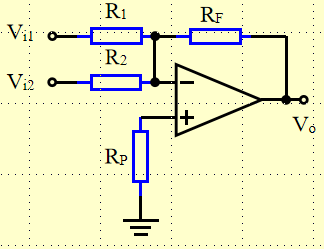
\includegraphics[width=0.4\textwidth, height=0.2\textheight]{figure/circuit_2.png}
    \caption{反相权重加法器电路}
    \label{fig:inverting_add_amp}
\end{figure}
当输入只有两个时，输出电压为 \(v_o = -R_f (\frac{v_{i1}}{R_1} + \frac{v_{i2}}{R_2})\)。

$R_p$一般取$(R_1||R_2)||R_f$，以减小输入偏置电流引起的运算误差。

若$R_1=R_2$，则$v_o = -\frac{R_f}{R_1}(v_{i1} + v_{i2})$，实现两个输入信号的反相加法运算。

若$R_1=R_2=R_f$，则$v_o = -(v_{i1} + v_{i2})$，实现两个输入信号的反相加法运算且无放大。

(3) \textbf{同相放大器}

\begin{figure}[H]
    \centering
    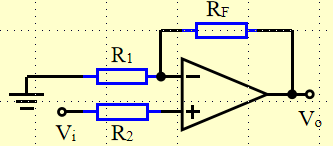
\includegraphics[width=0.4\textwidth, height=0.2\textheight]{figure/circuit_3.png}
    \caption{同相放大器电路}
    \label{fig:amp}
\end{figure}

	
	 电压增益 \(A_v\)： 根据“虚短”和“虚断”，对反相输入端节点列电流方程： \((0 - v_i)/R_1 + (v_o - v_i)/R_f = 0\)。解得：
	      \[
		      A_v = \frac{v_o}{v_i} = 1 + \frac{R_f}{R_1}
	      \]
	      输出电压与输入电压同相，且增益大于或等于1。

          输入电阻$R_i=\infty$

          输出电阻$R_o \approx 0$
	
$R_2$一般取$R_1||R_f$

若$R_1=\infty$，则有$v_o=v_i$，实现电压跟随功能。

(4) \textbf{减法器}

\begin{figure}[H]
    \centering
    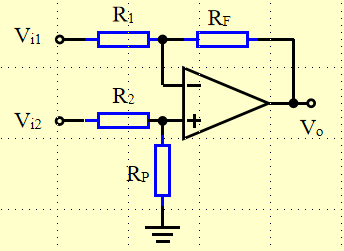
\includegraphics[width=0.4\textwidth, height=0.2\textheight]{figure/circuit_4.png}
    \caption{减法器电路}
    \label{fig:diff}
\end{figure}
由叠加定理得

\[V_o = \left( \frac{R_p}{R_2 + R_p} \cdot \frac{R_1 + R_F}{R_1} V_{i2} - \frac{R_F}{R_1} V_{i1} \right)\]

若电路对称，即：\( R_1 = R_2 \)，\( R_F = R_P \)，则

\[V_o = \frac{R_F}{R_1} (V_{i2} - V_{i1})\]


\section*{四、实验方案设计与参数计算}
(1) 反相放大器设计

设计反相放大器满足：电压增益$A_v=-15$，输入电阻$R_{in} \ge 15k\Omega$。

由于输入电阻$R_i \approx R_1$，可取$R_1=16k\Omega$。$R_f=|A_v| \times R_1 = 15 \times 16k\Omega = 240k\Omega$,$R_p=R_1||R_f=15k\Omega$

(2) 反相加法器设计

加法器满足$v_o=-(v_{i1} + 0.5v_{i2})$，并且$v_{i1}$为直流量，$v_{i2}$为交流量。

因此有电阻关系式$\frac{R_f}{R_1}=1$，$\frac{R_f}{R_2}=0.5$。
取$R_1=120\Omega$，$R_f=120\Omega$，$R_2=240\Omega$，$R_p=R_1||R_2||R_f=60\Omega$

仿真结果如图所示：
\begin{figure}[H]
    \centering
    \begin{subfigure}[b]{0.32\textwidth}
        \centering
        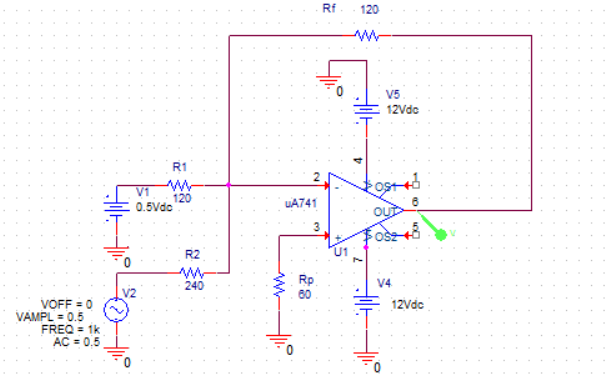
\includegraphics[width=\textwidth]{figure/sti/task2_cir.png}
        \caption{加法器仿真电路图}
        \label{fig:task2_sti_cir}
    \end{subfigure}
    \hfill
    \begin{subfigure}[b]{0.32\textwidth}
        \centering
        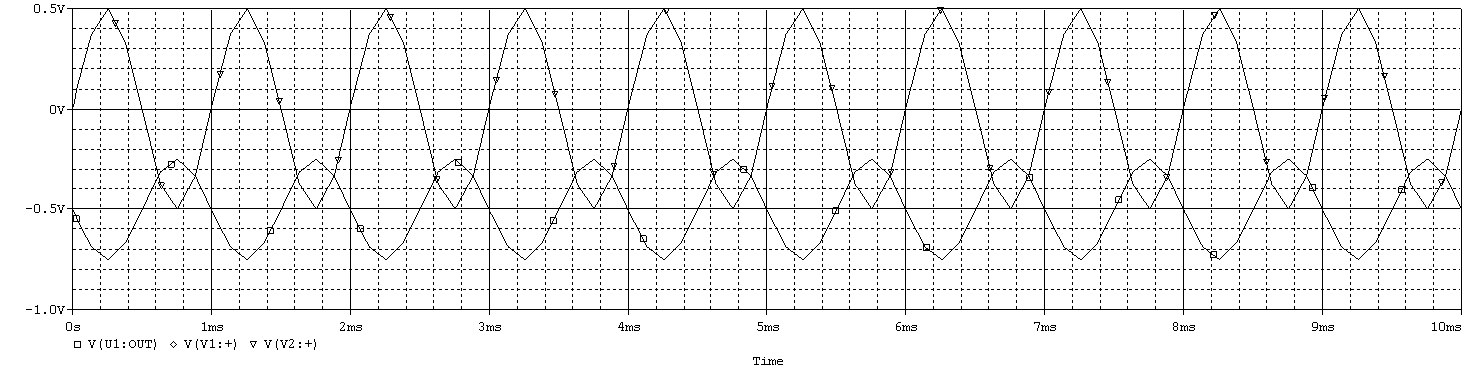
\includegraphics[width=\textwidth]{figure/sti/task2_img.png}
        \caption{加法器仿真波形图}
        \label{fig:task2_sti_waveform}
    \end{subfigure}
    \hfill
    \begin{subfigure}[b]{0.32\textwidth}
        \centering
        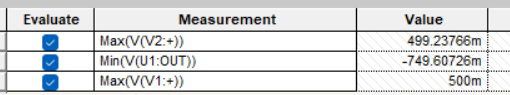
\includegraphics[width=\textwidth]{figure/sti/task2_mea.png}
        \caption{加法器仿真测量结果}
        \label{fig:task2_sti_mea}
    \end{subfigure}
    \caption{加法器仿真}
    \label{fig:task2_sti}
\end{figure}
根据测量结果，输入信号中直流量$v_{i1}=500mV$，交流量$v_{i2}$最大值为$499.23766mV$,输出量最小值$v_o=-749.60726mV$，

计算输出信号最小值应满足$v_o=-(v_{i1}+0.5v_{i2max})=-(500+0.5\times499.23766)mV=-749.61883mV$，与仿真值误差较小。表明电路设计正确。

(3) 增益带宽积测试电路设计
测试电路如下所示，分别改变$R_1$和$R_f$的值，测量不同增益下的截止频率，从而计算增益带宽积。
\begin{figure}[H]
    \centering
    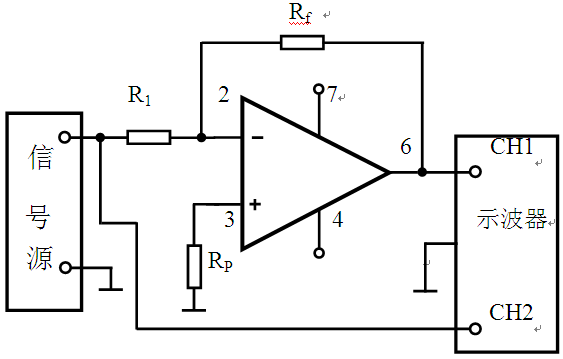
\includegraphics[width=0.4\textwidth, height=0.2\textheight]{figure/circuit_5.png}
    \caption{增益带宽积测试电路}
    \label{fig:GBW}
\end{figure}

仿真电路如下所示：
\begin{figure}[H]
    \centering
    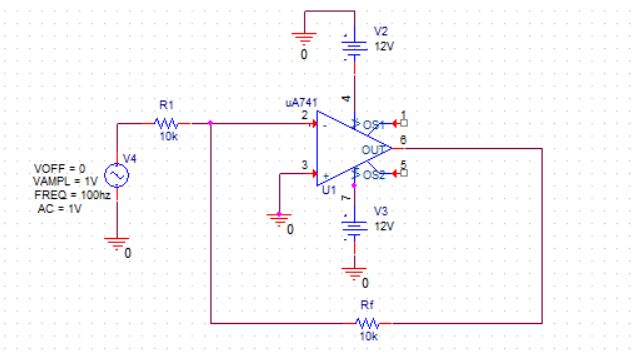
\includegraphics[width=0.4\textwidth, height=0.2\textheight]{figure/sti/task3_cir.png}
    \caption{增益带宽积仿真电路图}
\end{figure}

改变$R_f$的值，取$10k \Omega$,$100k \Omega$,$1M \Omega$三组参数进行仿真测试,
$R_f=10k \Omega$时仿真结果如图所示：
\begin{figure}[H]
    \centering
    \begin{subfigure}[b]{0.32\textwidth}
        \centering
        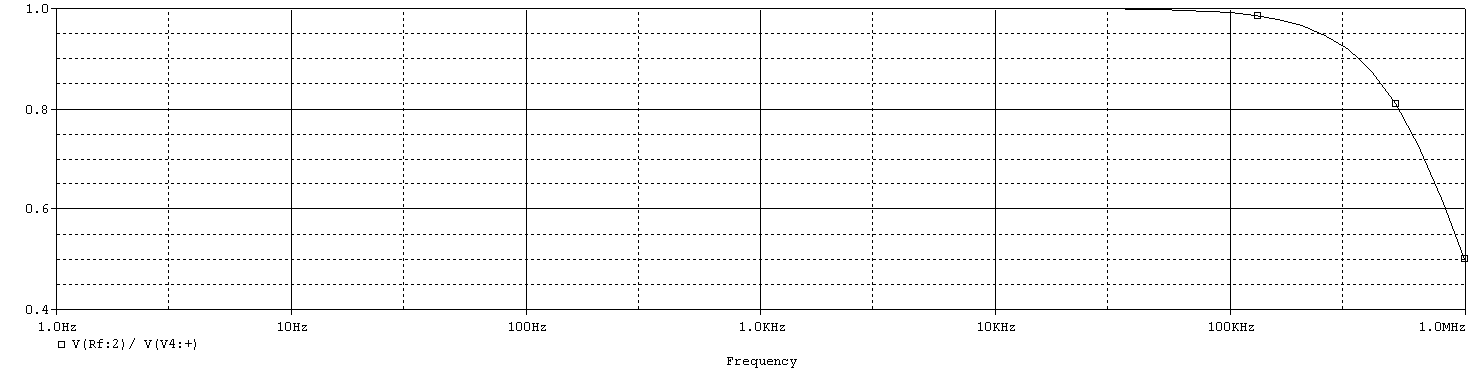
\includegraphics[width=\textwidth]{figure/sti/task3_1_wave.png}
        \caption{$R_f=10 k \Omega$时仿真电压增益频率特性曲线}
    \end{subfigure}
    \hfill
    \begin{subfigure}[b]{0.32\textwidth}
        \centering
        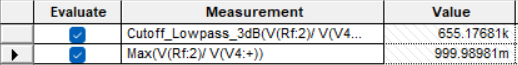
\includegraphics[width=\textwidth]{figure//sti/task3_1_mea.png}
        \caption{$R_f=10 k \Omega$时仿真电压增益与上限频率测量结果}
    \end{subfigure}
    \hfill
    \caption{$R_f=10 k \Omega$时仿真曲线与测量结果}
\end{figure}
根据测量结果，电压增益$A_v=1.00$，截止频率$f_H=655.18kHz$，计算增益带宽积$A_v \cdot BW=655.18 \times 10^3$。

$R_f=100k \Omega$时仿真结果如图所示：
\begin{figure}[H]
    \centering
    \begin{subfigure}[b]{0.32\textwidth}
        \centering
        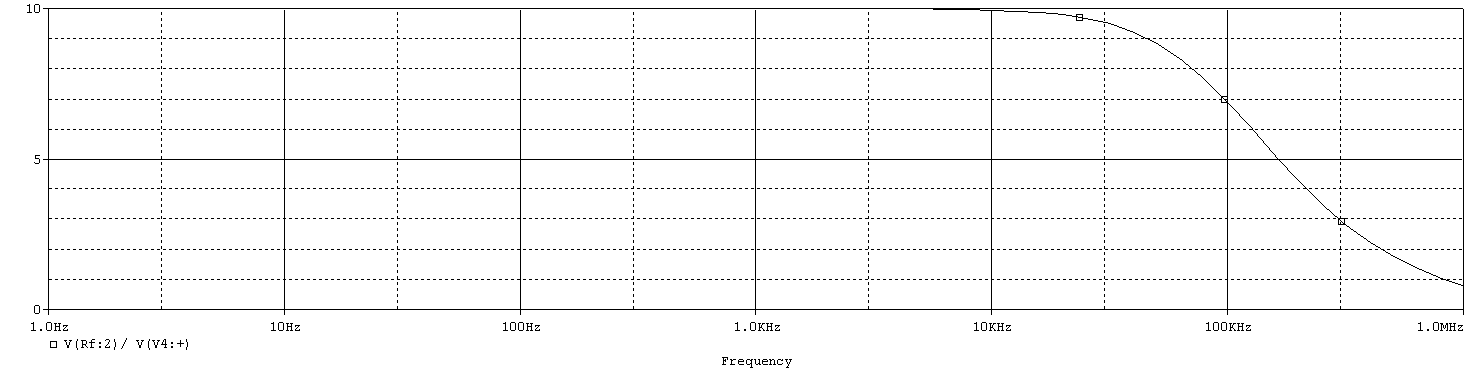
\includegraphics[width=\textwidth]{figure/sti/task3_2_wave.png}
        \caption{$R_f=100 k \Omega$时仿真电压增益频率特性曲线}
    \end{subfigure}
    \hfill
    \begin{subfigure}[b]{0.32\textwidth}
        \centering
        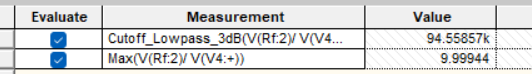
\includegraphics[width=\textwidth]{figure//sti/task3_2_mea.png}
        \caption{$R_f=100 k \Omega$时仿真电压增益与上限频率测量结果}
    \end{subfigure}
    \hfill
    \caption{$R_f=100 k \Omega$时仿真曲线与测量结果}
\end{figure}
根据测量结果，电压增益$A_v=10.00$，截止频率$f_H=94.56kHz$，计算增益带宽积$A_v \cdot BW=945.6 \times 10^3$。

$R_f=1M \Omega$时仿真结果如图所示：
\begin{figure}[H]
    \centering
    \begin{subfigure}[b]{0.32\textwidth}
        \centering
        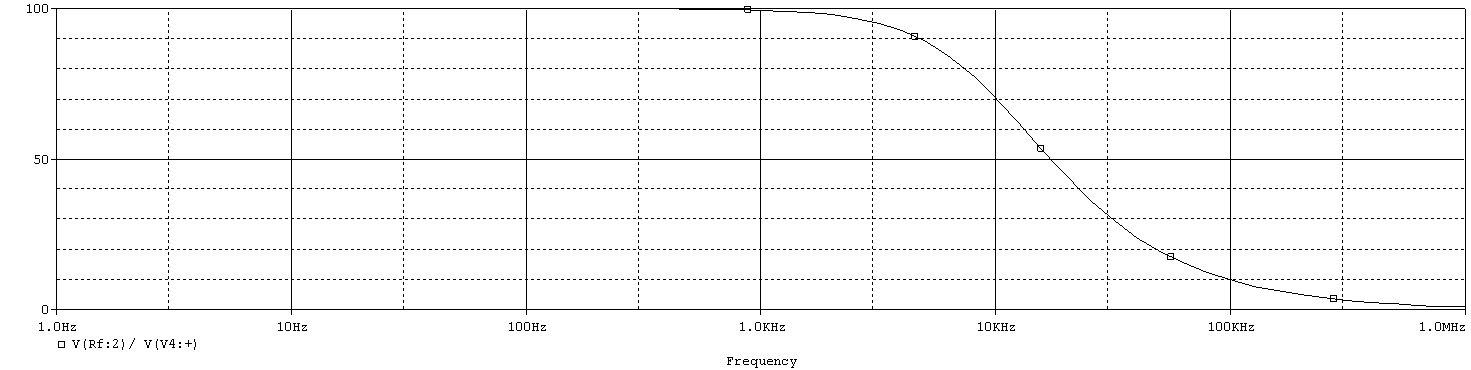
\includegraphics[width=\textwidth]{figure/sti/task3_3_wave.png  }
        \caption{$R_f=1 M \Omega$时仿真电压增益频率特性曲线}
    \end{subfigure}
    \hfill
    \begin{subfigure}[b]{0.32\textwidth}
        \centering
        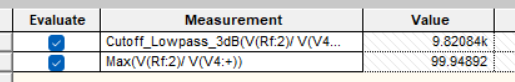
\includegraphics[width=\textwidth]{figure//sti/task3_3_mea.png}
        \caption{$R_f=1 M \Omega$时仿真电压增益与上限频率测量结果}
    \end{subfigure}
    \hfill
    \caption{$R_f=1 M \Omega$时仿真曲线与测量结果}
\end{figure}
根据测量结果，电压增益$A_v=100.00$，截止频率$f_H=9.82kHz$，计算增益带宽积$A_v \cdot BW=982 \times 10^3$。
根据仿真数据整理如下表格所示：
\begin{table}[H]
    \centering
    \begin{tabular}{|c|c|c|c|c|c|}
\hline & $R_{1}(\Omega)$ & $R_{f}(\Omega)$ &  $A_{v}$ & $f_{H}(kHz)$ & $A_{v} \cdot B W\left(\times 10^{3}\right)$ \\
\hline 1 & 10  k & 10  k  & 1.00 &655.18 & 655.18 \\
\hline 2 & 10  k & 100 k  & 10.00 & 94.56 & 945.6 \\
\hline 3 & 10  k & 1 M   & 100.00 & 9.82 & 982 \\
\hline
\end{tabular}
    \caption{增益带宽积仿真数据表}
    \label{tab:GBW_sti}
\end{table}
可以看到，增益带宽积基本保持不变，符合理论预期。
\section*{五、实验仪器设备}
电阻等电子器件，示波器，信号发生器，直流稳压电源，连接导线等。

\section*{六、实验步骤、调试过程、实验数据记录}
\subsection*{6.1 反相放大器电路搭建、测试}
搭建放大器电路并分别输入直流信号与交流信号，观察波形，计算电压增益。

输入直流信号时波形如下图所示：
\begin{figure}[H]
    \centering
    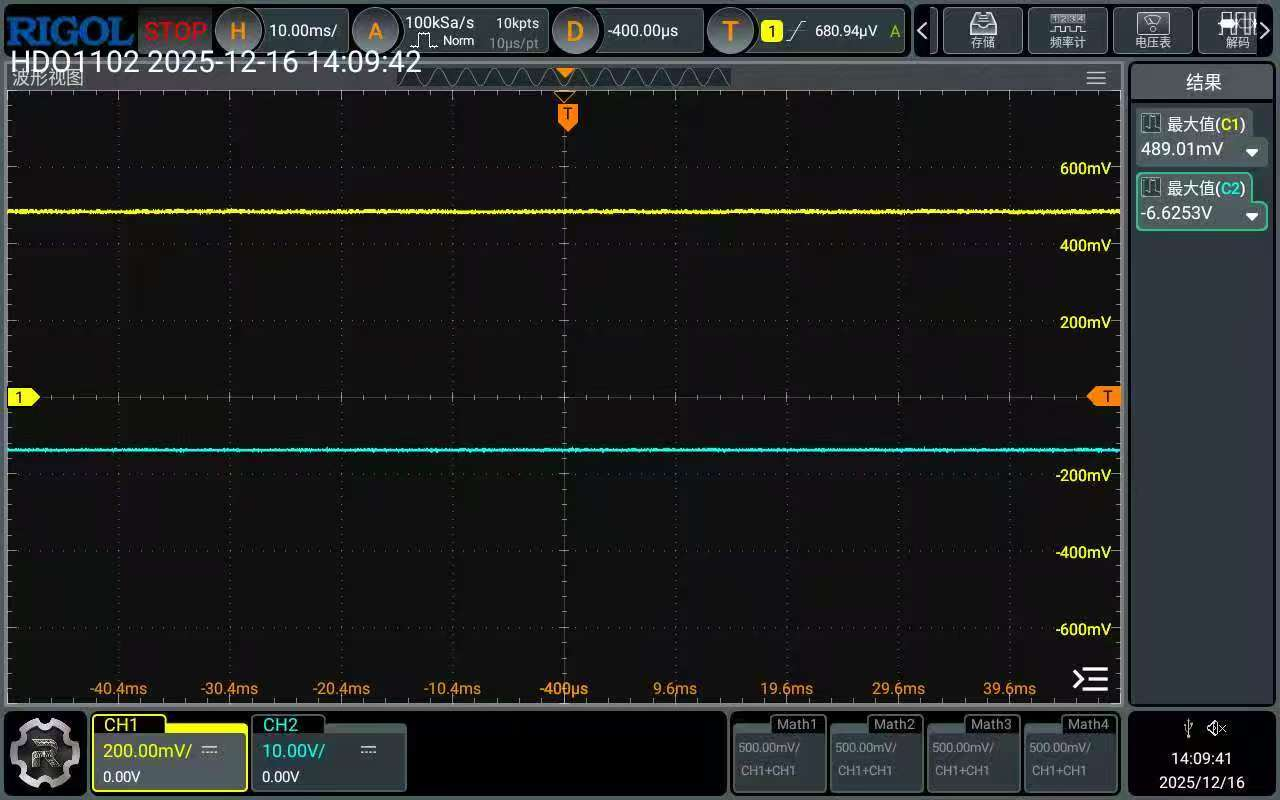
\includegraphics[width=0.4\textwidth, height=0.2\textheight]{figure//test/task1_dc.jpg}
    \caption{加法器直流输入时输出波形图}
    \label{fig:task1_dc}
\end{figure}
输入信号大小为$v_v=489.01mV$，输出信号$v_o=-6.6253V$，计算电压增益$A_v=\frac{v_o}{v_i}=-13.55$，与理论值误差较小。

输入交流信号时波形如下图所示：
\begin{figure}[H]
    \centering
    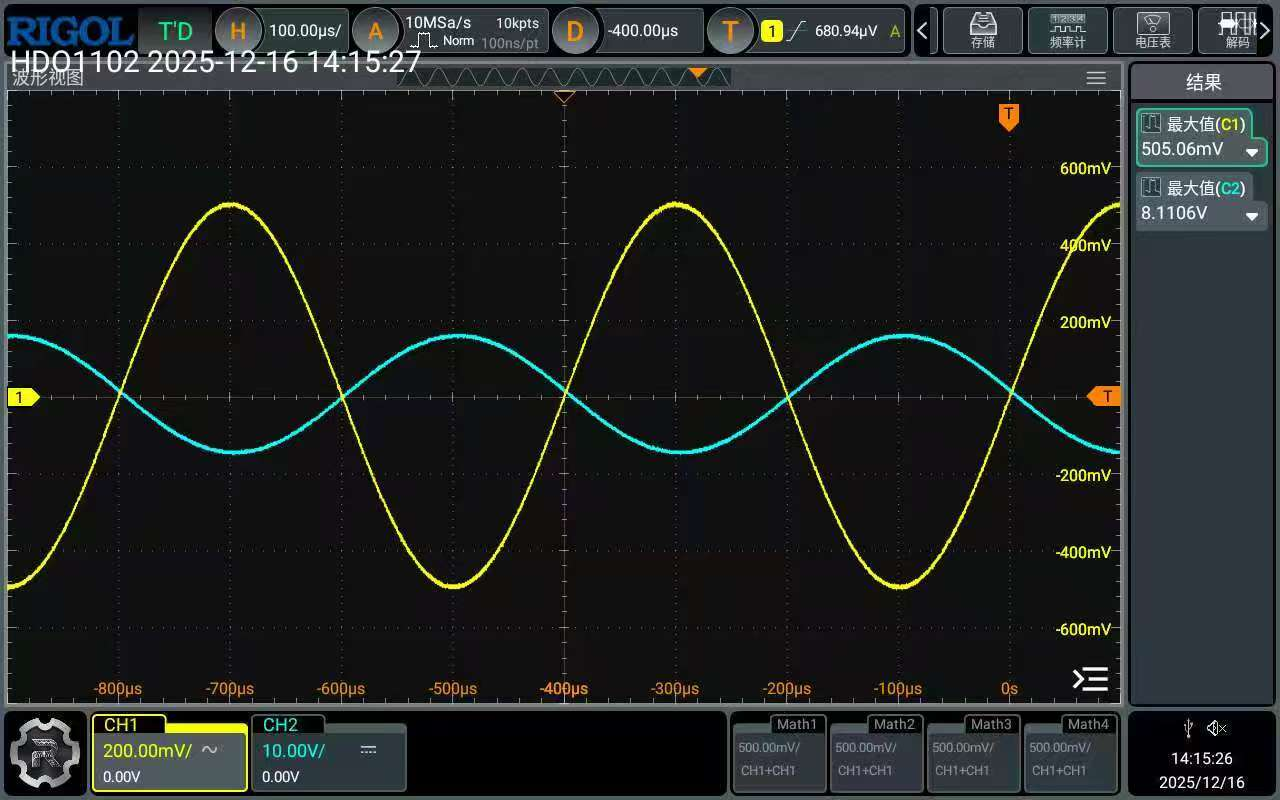
\includegraphics[width=0.4\textwidth, height=0.2\textheight]{figure//test/task1_ac.jpg}
    \caption{加法器交流输入时输出波形图}
    \label{fig:task1_ac}
\end{figure}
输入信号频率为2.5kHz，最大值为$v_{im}=505.06mV$，
输出信号最大值(大小最大)$v_{om}=-8.1106V$，计算电压增益$A_v=\frac{v_o}{v_i}=-16.06$，与理论值误差较小。
\subsection*{6.2 反相加法器电路搭建、测试}
搭建反相加法器电路，测量输入交流信号与输出信号波形如下图所示：
\begin{figure}[H]
    \centering
    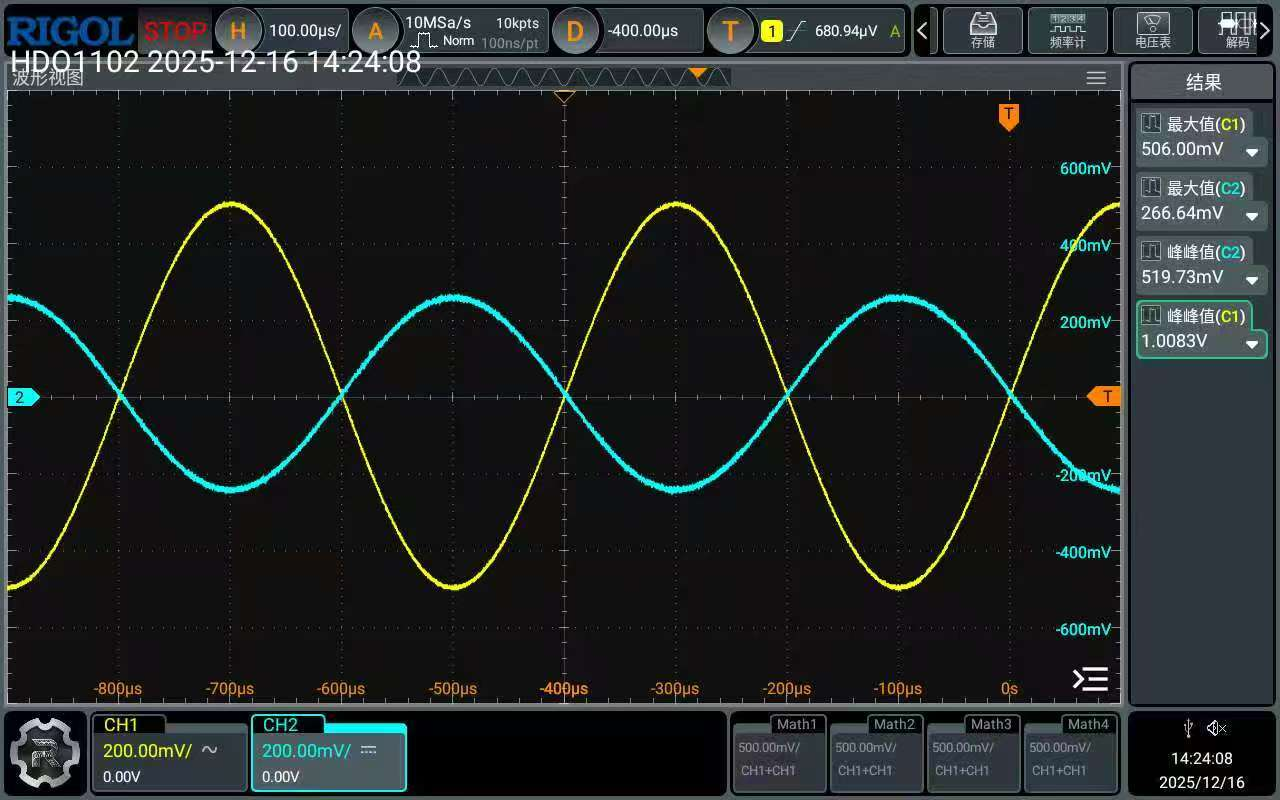
\includegraphics[width=0.4\textwidth, height=0.2\textheight]{figure//test/task2.jpg}
    \caption{加法器交流输入时输出波形图}
    \label{fig:task2_ac}
\end{figure}
输入信号中直流量$v_{i1}=503.1mV$，交流量$v_{i2}$峰峰值为$1.0083V$，最大值为$505.54mV$
输出信号峰峰值为$519.73mV$，最大值为$-238.7mV$，最小值为$-751.54mV$，计算输出信号最小值应满足$v_o=-(v_{i1}+0.5v_{i2max})=-(503.1+0.5\times505.54)mV=-755.87mV$，
与测量值$-751.51mV$误差较小。表明电路工作正常。
\subsection*{6.3 增益带宽积测试}
搭建增益带宽积测试电路，分别测量不同增益下的截止频率，计算增益带宽积，结果如下表所示：
\begin{table}[H]
    \centering
    \begin{tabular}{|c|c|c|c|c|c|c|c|}
\hline & $R_{1}(\Omega)$ & $R_{f}(\Omega)$ & $u_{i}(mV)$ & $u_{o}(mV)$ & $A_{v}$ & $f_{H}(kHz)$ & $A_{v} \cdot B W\left(\times 10^{3}\right)$ \\
\hline 1 & 10  k & 10  k & 102.77 & 101.88 & 0.99 &463.17 & 458.5383 \\
\hline 2 & 10  k & 100 k  & 57.373 & 587.06 & 10.23 & 149.74 & 1531.8402 \\
\hline 3 & 10  k & 1 M  & 74.008 & 7058.1 & 95.37 & 11.904 & 1135.28448 \\
\hline
\end{tabular}
    \caption{增益带宽积测试数据表}
    \label{tab:GBW}
\end{table}
可以看到，增益带宽积基本保持不变，符合理论预期。但是第一组数据与后两组数据差异较大，可能是由于测量误差引起的。
\section*{七、数据分析与讨论}

1. 反相放大器测试结果分析：

   直流输入时，实测电压增益 $A_v = -13.55$，与理论值 $-15$ 的相对误差为 $9.67\%$。

   交流输入时，实测电压增益 $A_v = -16.06$，与理论值的相对误差为 $7.07\%$。

   误差主要来源于电阻实际值与标称值的偏差、运放非理想特性以及测量仪器误差。

2. 反相加法器测试结果分析：

   实测输出电压最小值 $-751.54\text{mV}$，与理论计算值 $-755.87\text{mV}$ 的相对误差为 $0.57\%$。

   误差较小，表明电路设计合理，运放的虚短、虚断特性在实际电路中得到较好体现。

3. 增益带宽积测试结果分析：

   三组测量得到的增益带宽积分别为：$458.5\times10^3$、$1531.8\times10^3$、$1135.3\times10^3$。

   理论上增益带宽积应为常数，实测数据存在波动，尤其第一组数据明显偏小。

   可能原因：①低频测量时受环境噪声影响较大；②示波器测量误差，利用示波器测量电压增益与上限频率时误差较大

4. 实验现象与理论模型的差异：

   实际运放存在输入偏置电流、输入失调电压、共模抑制比有限等非理想特性，这些因素在高增益或高频条件下会影响电路性能。

   电路中使用的电阻存在精度误差（通常为$\pm5\%$），这也是实测结果与理论计算产生偏差的重要原因。

\section*{八、结论}

1. 成功设计并搭建了反相放大器、反相加法器和增益带宽积测试电路，各电路均能实现预期功能。

2. 实测结果验证了运放线性应用电路的基本原理：在深度负反馈条件下，运放工作在线性区，满足"虚短"和"虚断"条件。

3. 增益带宽积测试表明，运放的闭环增益与带宽成反比关系，增益带宽积基本保持恒定，验证了运放频率特性的基本规律。

4. 实验过程中也发现实际运放与理想模型存在差异，在高频或高增益应用时需要特别考虑运放的实际参数限制。
\section*{九、心得与体会}

1. 理论与实践相结合的重要性：通过本次实验，将理论课程中学到的运放理论知识应用于实际电路设计中，加深了对负反馈、虚短虚断等概念的理解。

2. 误差分析能力提升：实验中多次遇到实测值与理论值的偏差，通过分析误差来源，学习了如何从元件精度、测量方法、仪器误差等多方面考虑问题。

3. 电路调试技能提高：在搭建电路过程中，遇到输出波形失真、增益不准确等问题，通过检查电路连接、调整元件参数、优化测量方法等步骤解决问题，提高了实践能力。

4. 团队协作经验：与同组同学分工合作，一人负责仪器操作，一人负责数据记录，提高了实验效率，也学习了如何有效沟通协作。

5. 对运放实际应用的思考：认识到在实际工程设计中，不能仅仅依赖理想模型，必须考虑运放的失调电压、偏置电流、压摆率、增益带宽积等实际参数。
\section*{十、思考题}
1. 用运算放大器构成的负反馈电路其输出电阻可认为零，那么它能直接驱动电阻为$8 \Omega$的负载吗？为什么？

答：不能直接驱动。因为理想运放模型认为输出电阻为零，但实际运放的输出电阻虽然很小（通常几十欧姆），但并非真正为零。

几十欧姆的输出电阻会导致负载分得的电压过小，无法满足负载的工作要求。

2. 在同相电压跟随器电路中，设集成运放的最大输出电压为±12V，转换速率为$0.5\text{V/μs}$，输入正弦信号。当输入信号的频率为$1\text{kHz}$时，其最大不失真输出电压的幅度是多少？为了使最大不失真输出电压的幅度达到$8\text{V}$，信号的最高频率是多少？

答：
   对于正弦波$v_o = V_m \sin(2\pi ft)$，其最大变化率为$\left.\frac{dv_o}{dt}\right|_{\max} = 2\pi f V_m$。

   运放的转换速率SR限制了输出电压的最大变化率：$2\pi f V_m \leq \text{SR}$。

   当$f = 1\text{kHz}$时：$V_m \leq \frac{\text{SR}}{2\pi f} = \frac{0.5\times10^6}{2\pi\times1000} \approx 79.6\text{V}$。但受最大输出电压±12V限制，实际最大不失真幅度为$12\text{V}$。
   
   使$V_m = 8\text{V}$,则信号最大频率$f_{\max} = \frac{\text{SR}}{2\pi V_m} = \frac{0.5\times10^6}{2\pi\times8} \approx 9.95\text{kHz}$。

3. 反相比例放大电路中，电阻$R_1$的取值不可太小（如几十Ω），为什么？

答：
   输入电阻考虑：反相放大器的输入电阻$R_i \approx R_1$。若$R_1$太小，则输入电阻过小，会从信号源吸取过大电流，导致信号源负载过重，影响前级电路工作。

   功耗考虑：小电阻会导致电路功耗增大，可能引起电阻发热，改变阻值，甚至损坏元件。

   运放输出能力限制：$R_1$过小意味着反馈电阻$R_f$也相应较小（保持相同增益），导致运放需要提供较大输出电流，可能超出运放输出能力。

   一般$R_1$取几千欧到几百千欧为宜，既能保证足够大的输入电阻，又能避免上述问题。

4. 若要设计一个$A_{uf}=20$的同相放大电路，用于放大频率为$150\text{kHz}$的正弦信号，运放选用μA741可以吗？选用LM318可以吗？为什么？若放大频率为$1500\text{kHz}$的正弦信号呢？

答：
   首先计算所需增益带宽积：$\text{GBW} = A_v \times f_{\max} = 20 \times 150\text{kHz} = 3\text{MHz}$。

   μA741的增益带宽积典型值为$1.5\text{MHz}$，小于所需值，因此不适用于放大$150\text{kHz}$信号。

   LM318的增益带宽积典型值为$15\text{MHz}$，大于所需值，可以选用。

   对于$f=1500\text{kHz}$信号：所需$\text{GBW} = 20 \times 1500\text{kHz} = 30\text{MHz}$。
    μA741完全不能使用。
    LM318的GBW为$15\text{MHz}$，仍小于所需值，因此也不能使用。此时需要选择更高GBW的运放，如AD811（GBW约$140\text{MHz}$）。
\end{document}